\chapter{Contributions}

In the following sections, we present the main contributions related to the Train Benchmark framework.

\section{Disadvantages of the Train Benchmark Domain}

The original domain of the Train Benchmark framework (introduced in \ref{section:metamodel} is not applicable for our goals to analyze graph queries, and study model - performance relationships. The main problems connecting to the domain are summarized in the following list:
\begin{enumerate}
	\item The original domain is not related to a real-life model, which leads to the fact that the cardinalities of the elements and their relationships do not follow a real model's characteristic, therefore, the measurement results of different tools cannot be claimed to be representative in a real-life use case. \label{item:railway_problem1}
	\item Besides the origin of the domain, the second problem is that the artificially generated models do not cover a well-known topology or degree distribution that can be observed in actual networks. \label{item:railway_problem2}
	\item Finally, the generated models of Train Benchmark are not capable to attach arbitrary connections between the elements. \label{item:railway_problem3}
\end{enumerate}

Obviously, problem \ref{item:railway_problem2} is relevant to the generator component's insufficiency, since a representative distribution can be achieved independently on the domain, however, in order to generate arbitrary distributions, it is essential to guarantee a solution for problem \ref{item:railway_problem3}.

Problem \ref{item:railway_problem3} requires some explanation. In order to construct graphs with different degree distributions, it is an essential expectation of the domain to contain self-references, thus indicating that any of the vertices can be adjacent. In addition, the presence of a self-reference should be also interpretable conceptually in the domain. %todo kinda bullshit 

Considering the original domain, the type \textsf{Segment} represents the majority of the elements, however --- without breaking the original meaning of the domain --- we cannot make connection between any of the segments.
%todo well, rewrite this s**t later

To summarize, a new domain is necessary that is related to a real-life model, and also suited to use for generating different distributions.

\section{A Real-life Model}

For our purpose to analyze graph queries, we use a model of train schedules provided by the \textit{Network Rail} company that runs, maintains, and develops Britain's rail tracks~\cite{network_rail}. Network Rail publishes a number of different data available to developers, some of them are the following:
\begin{itemize}
	\item{Real-time train positioning and movement event data}
	\item{Performance of trains against the timetable, measured as the percentage of trains arriving at their destination on-time}
	\item{Daily extracts and updates of train schedules}
\end{itemize}

The most adequate data for our aim is the daily schedules of trains, hence, the performance analysis is also based on this data.

\subsection{An Overview of the Train Schedules Data}\label{sec:schedules_overview}
The data of schedules can be divided into three different types of records\footnote{In the data of schedules a record actually represents a JSON object.} that are defined hereunder~\cite{schedules_data}:
\begin{itemize}
	\item{\textit{Association records}}: indicate the relationships between trains.
	\item{\textit{Schedule records}}: refer to the train schedules themselves.
	\item{\textit{Tiploc records}}: include information about timing point locations in the schedules.
\end{itemize}

At first, note that the trains themselves do not appear in a distinguished type of record, with the exception of their identifiers (\textit{Train UID}) that can be found in the association and schedule records, therefore, the data lacks of any information that describes the attributes of the physical trains.

An association is interpreted between two distinct trains that are somehow interconnected belonging to the same and only one location. For example, a dividing association means that a train separates into an other one in a particular station~\footnote{From now on, we use the words location and station as synonyms.}. However, an association does not necessarily occur, since there are trains that are not associated to any. To summarize, an association record always belong to the distinct trains, and one location.

A schedule record attaches locations to a certain train, thus, it defines a path of locations, which are divided into three different groups in a schedule, representing their positions in the path such as \textit{origin}, \textit{intermediate}, or \textit{terminating} location. One schedule always belongs to one train, even though a train can be referred by more schedules as well, and obviously, more than one schedule can include the same location.

Finally, \textit{Tiploc records} contain the locations.

\subsubsection{Cardinalities}

The data of schedules in Network Rail typically contain daily representations of the trains, however, an entire data model is available as well that contains every schedule information for each day. Since it includes a significantly larger data, from now on, we rely on this in our benchmark framework.

In the entire data, the cardinalities belonging to the individual types are depicted in Figure 1. %todo create a pie chart of cardinalities per entities
As can be observed, schedules represent the majority of the records, furthermore, only a small set of trains\footnote{Since train records are not defined in the data, in this case the number of trains are equal to the number of distinct train identifiers.} are in any kind of association with another train. The cardinality of locations indicates the number of unique locations, instead of their cumulated appearances. Regarding the latter, approximately 5.8 million number of locations occur as destinations attached to the schedules. It leads to the fact that the average number of attached destinations to a schedule is $15.66$.

\subsection{Mapping to a Model}\label{sec:mapping_schedule}

The previously introduced data of train schedules must be transformed to a graph on which the measurements can be accomplished. The corresponding domain derived from the data is depicted in Figure 2. %todo add a mesmerizing metamodel, or ER diagram and some footnote:this is actualy represented in blah blah to clarify blah blah
%todo don't mix the concepts of graph and metamodel, or domain and model, use a consistent expression
By mapping the domain to a graph leads to four different types of vertices: \textsf{Association}, \textsf{Station}, \textsf{Schedule}, and \textsf{Train}. The station symbolizes the location, and the references --- such as \textsf{association}, \textsf{associative}, \textsf{destinations}, and so on --- follow the same approaches introduced in Section \ref{sec:schedules_overview}, and they are mapped to directed edges in the graph. 

One newly introduced edge is the \textsf{neighbor} connection among the stations. The presence of a \textsf{neighbor} edge between two stations implicates the existence of a path from the first station to the second via the same schedule, and these stations follow each other in the schedule's destinations. In other words, the consecutive stations from a schedule's path become adjacent. Figure 3 demonstrates an example which nodes of stations are connected via \textsf{neighbor} edges, assuming that originally those locations belonged to the same schedule. As a conclusion, \textsf{Station1} and \textsf{Station2} are connected since they are adjacent in the destinations of \textsf{Schedule1}, on the contrary, \textsf{Station1} and \textsf{Station3} are not drawn to each other, since they are not consecutive stations among the schedule's destinations, despite the fact that both of them can be found in it. %todo draw a graph
Important to note that more than one adjacency in different schedules's stations do not implicate more \textsf{network} edges between the nodes.

\subsubsection{Attributes}

As can be observed in Figure 2, %todo add pic reference
there are different attributes belong to the vertices that can be found in the original data set as well. These attributes are briefly introduced below:
\begin{itemize}
	\item{\textsf{Schedule Planning}}: It can be \textit{Short-term}, or \textit{Permanent}.
	\item{\textsf{Status}}: It indicates the train status, and its possible value comes from the following enumeration: \textit{Freight}, \textit{Passenger}, \textit{Ship}, \textit{Bus}, and \textit{Trip}. Since a schedule can be a short-term overlay, thus, a temporary schedule may belong to a substitute bus or ship.
	\item{\textsf{Days}}: A seven-character binary variable, the first represents Monday, and last one is Sunday. For example, the attribute for a schedule --- that runs on every Monday and Sunday --- is equal to \textit{1000001}.
	%todo stpindicator is missing yet
	\item{\textsf{Start Date}}: The start date of the schedule.
	\item{\textsf{End Date}} : The end date of the schedule.
	\item{\textsf{UID}}: The unique train identifier.
	\item{\textsf{Category}}: Refers to the association's category that can be \textit{Divide}, \textit{Join}, \textit{Next}.
\end{itemize}
%todo mark that attributes with bold which will be used in the queries


\subsection{Model Analysis}\label{sec:model_analysis}
cardinalities
	prob distr
	scale-free, power-law dist
	random schedule factor -> important?


\section{Extending the Framework with Analysis}
\subsection{Metrics Calculation}
\subsubsection{Model-related Metrics}
\subsubsection{Query-based Metrics}
\subsection{The New Architecture of the Framework}
components and shit
+ dynamic query builders
\subsection{Workflow}
phases and shit

\subsection{Regression Analysis}

\subsubsection{MARS}


\section{Model Generation} 

The following sections represent the concepts of a new model generation that is elaborated in the Train Benchmark framework.
\subsection{Concepts}
The fundamental goal in Train Benchmark is to generate arbitrary, dynamic models with different structures, and various degree distributions. As Section \ref{sec:benchmark_conclusions} emphasizes, all of the well-known RDF benchmarks rely on static models, and they only propose one particular structure in various sizes. Our aim is to approach the performance analysis from a new aspect by focusing on the internal structure of the model, and investigating its effect to the performance.

\subsection{Overall of the Generation Steps}
The new generation mechanism in Train Benchmark is based on the \textit{Schedule} model, introduced in Section \ref{sec:mapping_schedule}, and it can be divided into different steps which are depicted in Figure 1. %todo add generation steps figure
The necessary steps are described hereunder:
\begin{enumerate}
	\item The network among the stations is generated. This graph's characteristic can follow various degree distributions, as its structure is shaped via different well-known graph topology algorithms.
	\item The generator creates schedule vertices and links stations to them, thus, they symbolize the destinations in each schedule's path.
	\item The generator instantiates the train nodes and attaches them to the schedules so that every schedule has a connection with a train.
	\item The attributes are initialized and linked to the nodes. The values of the variables are determined by following the same distributions found in the original data. As a consequence, as many --- for example --- short-term schedules are in the generated graph as appeared in the original real-life data as well, by considering the same size.
	\item A connectivity check is executed on the graph.
	\item Finally, the model can be persisted to the particular tool's format.
\end{enumerate}

\subsection{Topologies}
The most flexible part in the artificially generated models is the network among the stations, as using various well-known graph topologies we can change the internal structures of the network, and thus, obtain different degree distributions. The utilized topologies are the following:
\begin{itemize}
	\item Random Graph
	\item Watts-Strogatz Model
	\item Scale-free Networks of Barabási-Albert
	\item Hierarchical Network
\end{itemize}
The models and their algorithms are introduced in Section \ref{sec:topologies}, therefore, this section only includes the specific information about the .

\subsubsection{Random Graph}
From the two known algorithms, Gilbert's $G(n,p)$ model is adapted to the framework.

\subsubsection{Watts-Strogatz Model}\label{sec:watts_generation}

The commonly known generation algorithm is used with some extensions. Generally, the $N$ value in the algorithm --- that represents the number of consecutive connected nodes --- is a constant, which indicates a liner relationship between the number of edges and nodes, since every vertex has $N$ degree. However, we extend the algorithm by defining an inclusive lower ($N_1$) and upper ($N_2$) bound for $N$, as $N\in[N_1, N_2]$, and also assign a probability to $N$ that determines the number of consecutive interconnected nodes to be $N_1$ or $N_2$. As a result, this conducts to a generation that can obtain a more flexible, non-linear relationship between the number of edges and nodes.

\subsubsection{Scale-free Networks of Barabási-Albert}

In the original generation algorithm, every new vertex becomes to be connected to a constant number of disjunct nodes. Similarly to the notion in the Watts-Strogatz model generation (\ref{sec:watts_generation}), this constant value is converted to a random variable by a particular probability.

\subsubsection{Hierarchical Network}\label{sec:hierarcical_contribution}

The first difference between our constructed hierarchical graph and the original concept is that the former structure can be configured arbitrarily, since it is feasible to create $K_n$ complete subgraphs with optional $n$, instead of $K_5$. %todo use this notation in background too

The second most essential difference is the termination of the generation algorithm. As a general rule, the goal in Train Benchmark is that to generate arbitrary size of models by creating a precise number of nodes. Since the generation of hierarchical network is recursive instead of being incremental --- as in the case of the three other topologies --- it is inevitable to determine a termination from the recursion. The termination point is evident, as soon as the number of created nodes reaches the limit, the algorithm has to be stopped. However, it cannot be predicted in which phase the algorithm stops exactly. As a consequence, the possible failures have to be managed.

\begin{figure}[!ht]
	\centering
	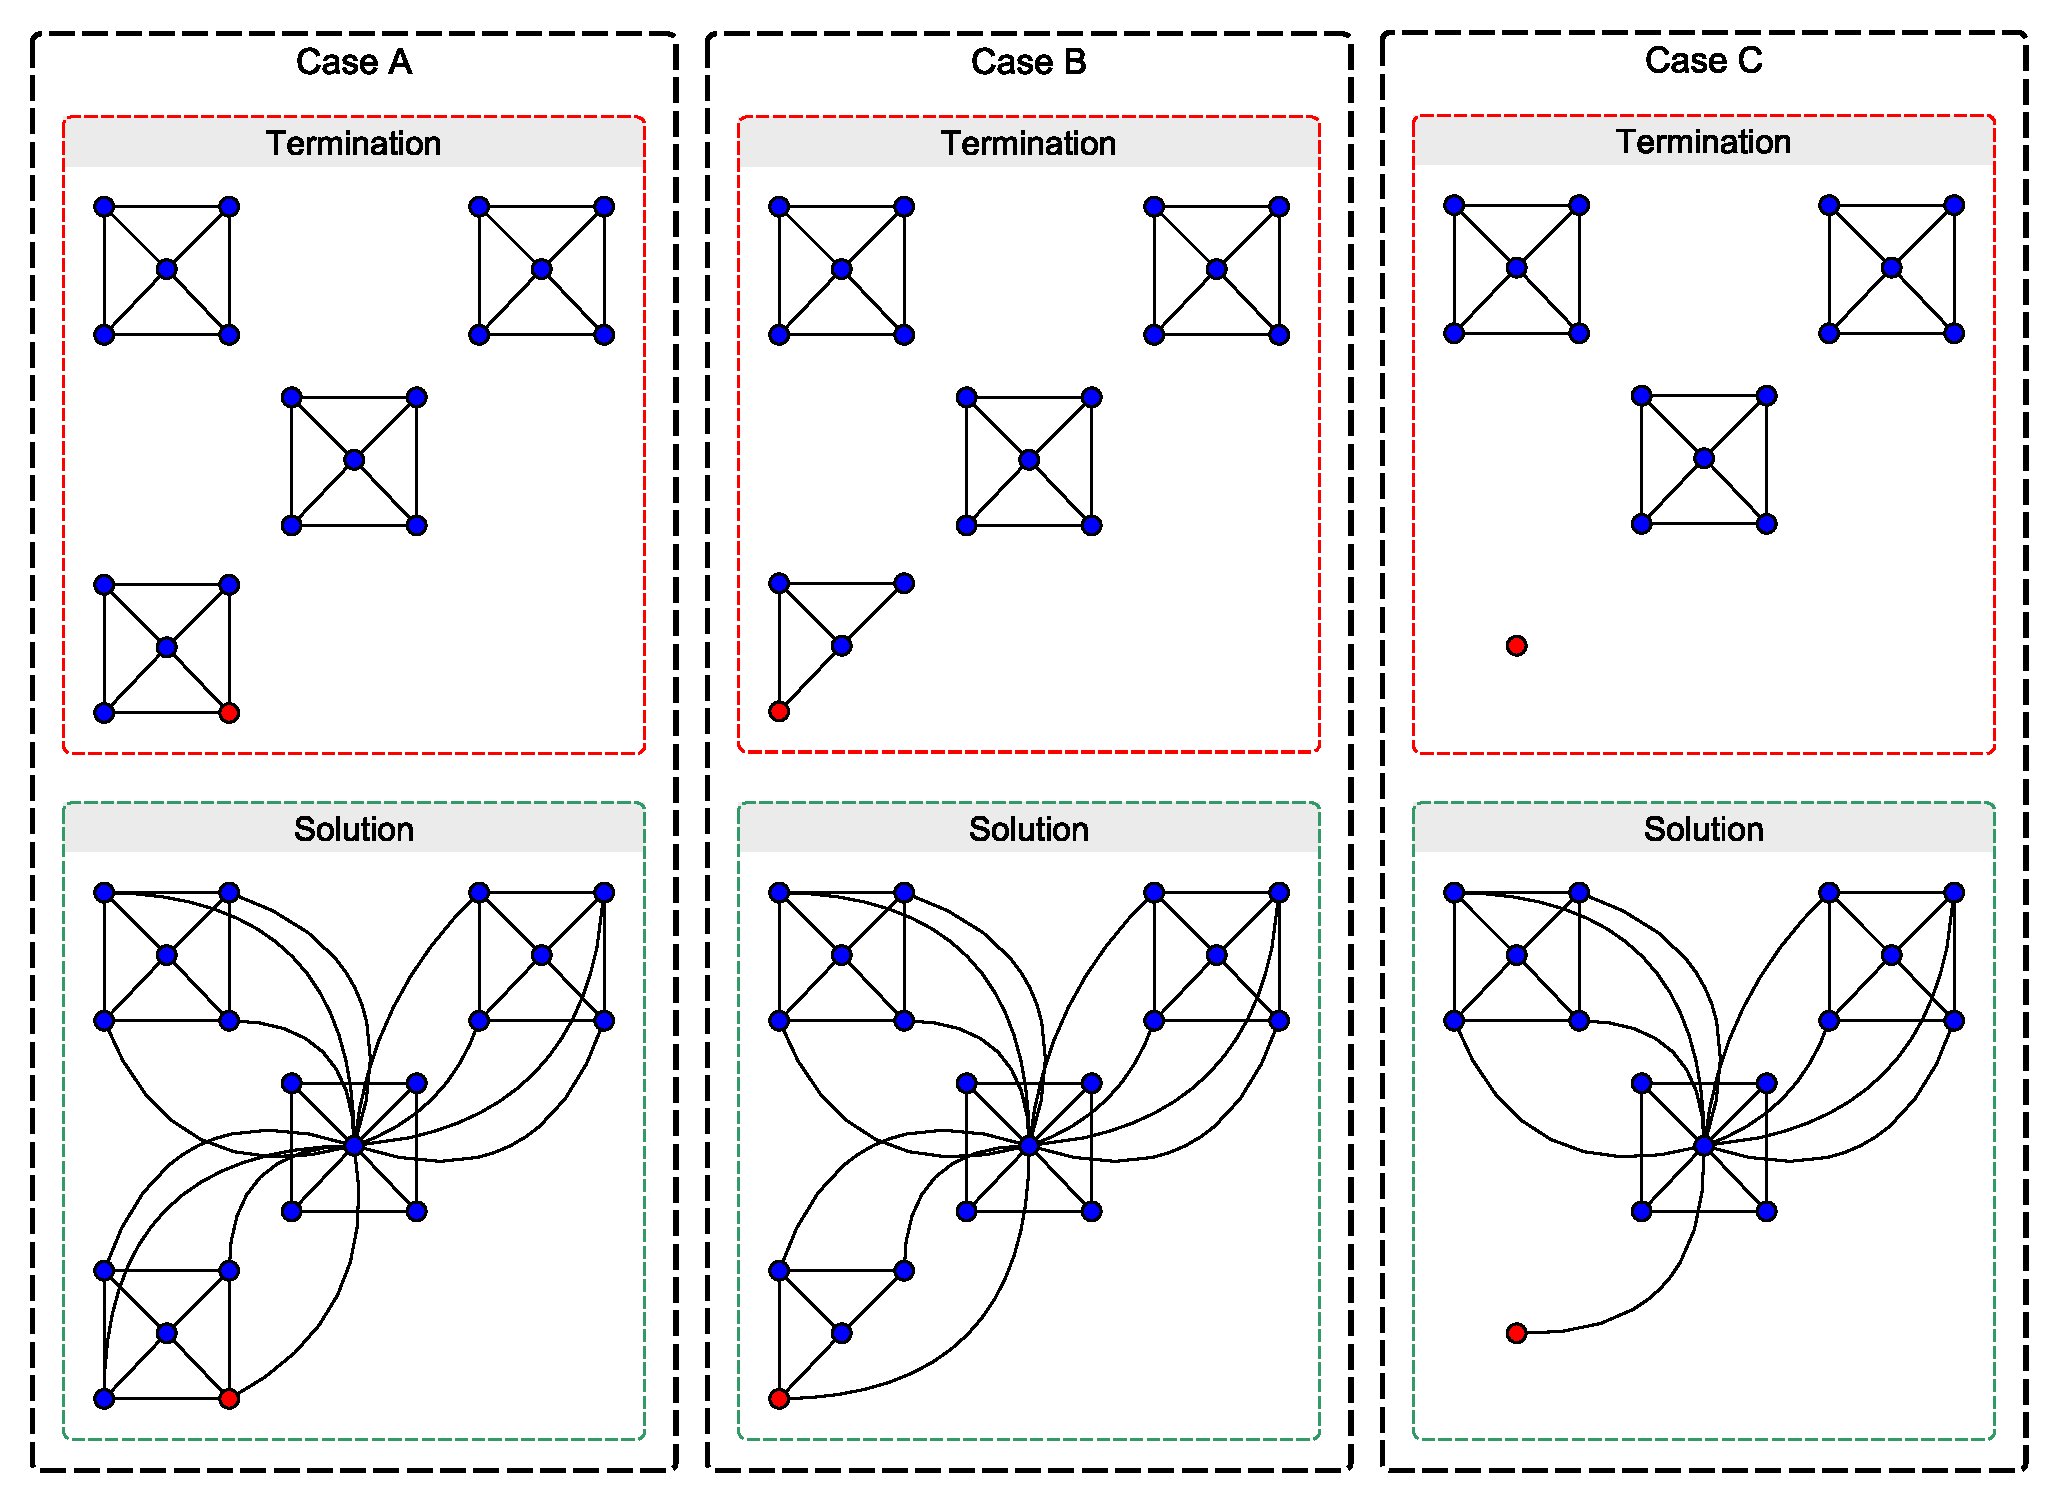
\includegraphics[width=150mm, keepaspectratio]{figures/hierarchical.pdf}
	\caption{Termination problems in hierarchical graph generation}
	\label{fig:hierarchical_problems}
\end{figure}

The possible problematic cases are demonstrated in Figure \ref{fig:hierarchical_problems}. In \textsf{Case A}, \textsf{B}, and \textsf{C}, the expected numbers of nodes are 20, 19, and 16, respectively. As it can be observed in these cases, this limit is always reached before the fourth cloning occurs, since 5 clusters should be created with 25 vertices at the end of this step in the recursion.

In the solution in \textsf{Case A}, the generator stops the clone procedure and connects the diagonals to the center. Regarding \textsf{B}, the termination happens during the generation of a cluster. As a solution, the last cluster becomes partial, and similarly, every diagonal is attached to the center. \textsf{Case C} represents that scenario when the last cluster only consists of one node. To prevent isolation, the last vertex is considered as a diagonal, and be connected to the center.

\subsection{Schedule Connections}\label{sec:schedule_connections}

An important part of the generation is that to connect the stations to schedules. As it was detected in Section \ref{sec:model_analysis}, the degree distribution of the schedule and station connections follows a power-law distribution. %todo add exponent value

In order to simulate a similar characteristic, we generate a power-law distribution from a uniform distribution~\footnote{It is a more convenient way to use an uniform distribution that is easier to be accomplished due to a built-in random generator.} with the following formula~\cite{power_law_from_uniform}:
\begin{align}
	X = \Big[\big(x_1^{(n+1)} - x_0^{(n+1)}\big)y + x_0^{(n+1)}\Big]^{(\frac{1}{(n+1)})}
\end{align} 
where $n$ is the exponent or scale-factor, $y$ is a uniformly distributed variate on $[0,1]$, and $x_0$, $x_1$ are the minimum and maximum bounds of the interval. Finally, $X$ is determined for every schedule, and it represents the number of stations that have to be connected to the certain schedule. Due to this solution, the schedule and station connections show a power-law characteristic.

Another problem is choosing the appropriate stations. Actually, the value of $X$ is the length of the destinations path belonging to a schedule. As a result, for every schedule, the generator executes a \textit{breadth-first search} starts from a uniformly random station, and stops the algorithm as soon as it finds an $X$ length path. Finally, this path of stations is linked to the schedule.


\subsection{Possible Model Configuration}

In an artificially generated model, the cardinality, size, topology, and density is optionally configurable. 

Regarding cardinality, different proportions can be adjusted between the vertex types, as \textsf{Station}, \textsf{Schedule}, \textsf{Train}, and \textsf{Association}. The default adjustment is proportional to the observed cardinality in the case of the original data.

The size of the model --- so the number of nodes --- is calculated as $|V| = s \cdot 2^i$, where $s$ is the step size constant, $5000$ by default, and $i$ is a positive integer, given by the user.

As it was already emphasized, various graph topologies can be generated among the \textsf{Station} nodes, thus, the internal structure of the models and their degree distributions are also alterable. Moreover %todo finish

\subsection{Uniform Model Generation}

In the generation unit in Train Benchmark, it became possible to construct \textit{uniform} models with various topologies. Under the concept of uniformity, it is meant that the different models may consist of some particular \textit{static} subgraphs that are found in each one, furthermore, the models include the same number of nodes and edges, regarding the \textit{dynamic} parts, thus, the topologies as well.

%todo add a figure

\subsubsection{Static Subgraphs}
Regarding the static parts, the ensemble of \textsf{Train} and \textsf{Association} types of vertices can be classified to this category. Obviously, if the cardinality configurations --- the proportion of the elements --- in the models are the same, than these types of nodes and their relationships are equal, since they are generated by the same algorithm.

In terms of the \textsf{Schedule} nodes, achieving a completely uniform subgraph between the schedules and stations is not feasible. At first, note that those stations that are linked to the schedules, are chosen via a breadth-first search algorithm, which implicates different paths of destinations for the schedules in each model depending on the topology among stations. As a result, a precise, uniform internal structure between the schedules and stations cannot be generated, however the average degree of a \textsf{Schedule} node --- thus, the amount of corresponding destinations --- is precisely configurable, since the degree distribution of schedules is determined forward by a power-law generator (introduced in Section \ref{sec:schedule_connections}), yet, this configuration entails a problem.

The problem is the maximum size of paths among stations, reached by the BFS algorithm. Even though the Scale-free, random, and Watts-Strogatz models can be considered as arbitrary connected graphs, which leads to the assumption that a path exists among any two nodes with an optional length. However, this statement cannot be claimed in the case of hierarchical networks. There always exists a path between two arbitrary nodes in a hierarchical graph via the \textit{center node}\footnote{It is actually the first created node in algorithm, and in the further steps every diagonal is linked to this vertex.}. However, the maximum depth in this path without revisiting the center node again, is bounded. It is easy to confirm, since the sub hierarchies are not connected explicitly to each other, expect the center node. As a consequence, the maximum length between two nodes --- considering the best scenario --- consists of $\frac{|V|}{2^i}$ nodes, where $i$ is the current iteration value of the recursive algorithm. Considering an average case, the maximum length is $\frac{|V|}{2 \cdot 2^i}$. According to this number, the maximum bound of the power-law generation function is adjusted.

Note that, by achieving uniformity among the models, as using a consistent degree distribution in schedules based on the hierarchical graph, the generated models loose some of their real-life characteristics that was observed it the original data.

\subsubsection{Number of Nodes}

The question of nodes equality per graphs is related to the \textit{dynamic} parts of the graph, thus, to the topologies among the stations.

The only one problem about generating a graph with a certain number of nodes is the recursive algorithm of the hierarchical graph. Nevertheless, we already showed in Section \ref{sec:hierarcical_contribution} that the recursion is terminated appropriately, and the resulting problems are managed.

As far as the other structures are concerned, the ensemble of random graph and the Watts-Strogatz model is constructed by initializing $|V| = N$ number of vertices at first, and subsequently, the algorithms determine which one of them become adjacent. In the scale-free model generator, the nodes are created incrementally until $|V| = N$. As a deduction, a precise number of nodes in these topologies to be uniformed can be achieved easily.

\subsubsection{Number of Edges}

The only one challenge of obtaining an equal number of edges among the models is related to \textit{dynamic} parts of the graphs, the topologies. As it was already emphasized, the random graph, Watts-Strogatz model, and scale-free network can be configured optionally, which conducts the fact that arbitrary number of edges can be generated, even the same amount for every topology. Actually, in these types of networks, the amount of nodes and edges are handled respectively.

Unfortunately, the creation of nodes and edges in the hierarchical graph occurs together. Since generating of a certain number of nodes, $|V|$is already handled, the key is to find a relationship between $|E|$ and $|V|$.

The literature relating to hierarchical graphs does not study the exact number of edges or its correlation to the amount of nodes, hence, we propose a solution to estimate $|E|$ in the recursive algorithm for every iteration.

At first, let define the necessary variables hereunder:
\begin{itemize}
	\item{$i$}: Represents the current iteration in the original hierarchical algorithm.
	\item{$c$}: Indicates the number of clones in every iteration.
	\item{$n$}: The cluster size is denoted by $n$, which cluster is a $K_n$ complete graph.
	\item{$F_i$}: It indicates the constructed graph after the $i$ iteration.
	\item{$|E_{F_i}|$}: The number of edges of the $F_i$.
\end{itemize}

In the 0. iteration, the hierarchical graph consists of one $K_n$ cluster. Formally speaking, $F_0 = K_n$, and $|E_{F_0}| = |E_{K_n}| = \frac{n \cdot (n-1)}{2}$. In the 1. iteration, the algorithm clones $F_0$ for $c$ times, and connects the diagonals from each $F_0$ to the center node. It entails that 
\begin{align}\label{eq:f1_version1}
	|E_{F_1}| = (c+1) \cdot K_n + c \cdot (n - 1)	
\end{align}
since $c+1$ number of $K_n$ can be found in $F_1$, and $c \cdot (n - 1)$ edges can be drawn from the $c$ cloned clusters to the center.

Note that $K_n$ can be substituted with $F_0$, furthermore, the algorithm connects $c^i$ clusters to the center, which implicates $c^i \cdot (n-1)$ diagonals, and edges as well. Thus, modifying Equation \ref{eq:f1_version1}, we obtain:
\begin{align}\label{eq:f1_version2}
	|E_{F_1}| = (c+1) \cdot F_0 + c^1 \cdot (n - 1)	
\end{align}
Generally, derived from Equation \ref{eq:f1_version2} the formula for every iteration is the following:
\begin{align}
	|E_{F_i}| = (c+1) \cdot F_{i-1} + c^i \cdot (n - 1)	
\end{align}


\section{The Workloads for Graph Queries Analysis}

\subsection{Main Goal}
investigate stations
\subsection{Sample Choosing}
which topologies? in what proportion?
\subsubsection{A Sample Based on Topologies}

plot metrics low deviation -> kick random

\subsubsection{A Sample Based on Metrics}
+ fig reference about WS from BA
plot metrics -> high deviation, that's it -> we are happy

\subsection{Model Configuration}
change cardinality and shit
\subsection{Evaluated Queries}

\subsubsection{Transitive Closure}
oh we love it
property path * operator
add sparql query
\subsubsection{Navigations}
\subsubsection{Attributes}
\subsection{Investigated Tools} briefly
which can be used for Q1, Q2, Q3? 
1 sentence description about them not so interesting but important
